\documentclass[a4paper,12pt,twoside]{article}
\usepackage{IEM_2nd_Qtr}



\begin{document}

\thispagestyle{empty}

\begin{center}
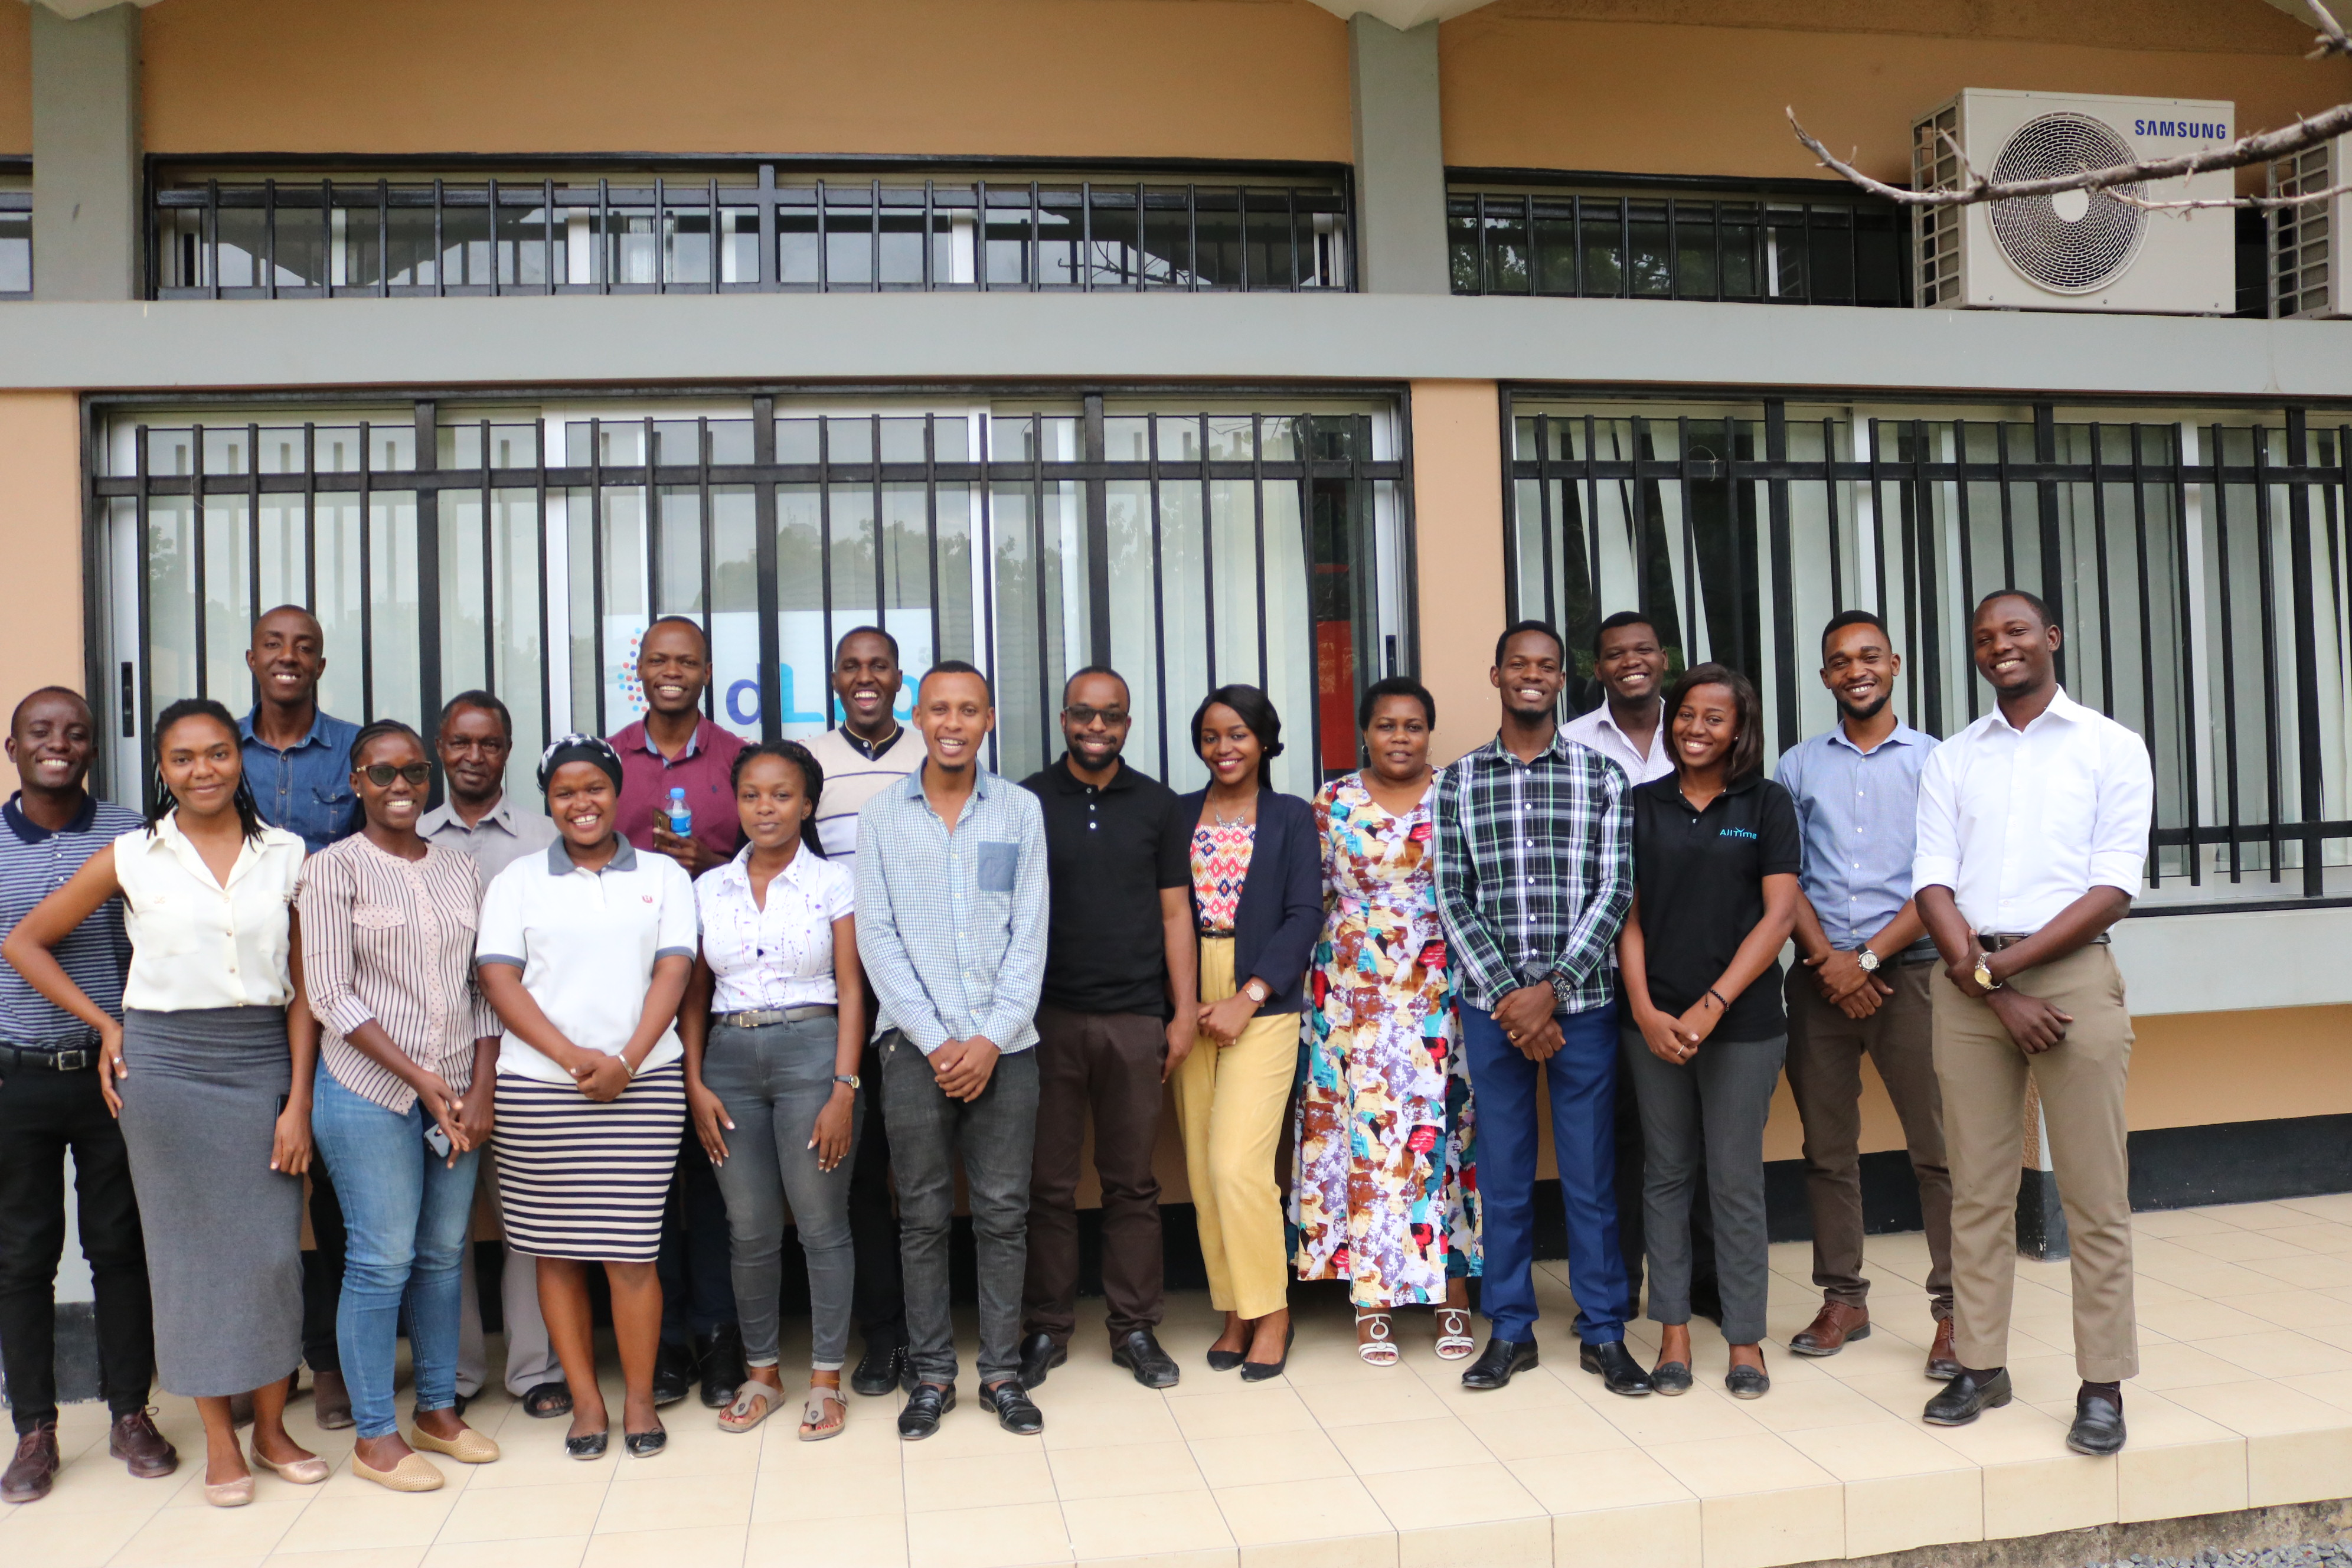
\includegraphics[width=\textwidth]{Group_shot.JPG}
\end{center}

\begin{center}
\bigskip
  \Huge 
\color{OMDTZblue} \textbf {Innovation Ecosystem Map}
\\
\textbf{Project Progress Report}
\\
\end{center}
\bigskip \bigskip \bigskip
\\
  \vbox{
  \centering
  Prepared for:
  \vcenteredhbox{
\includegraphics[width=2cm]{images/hdif_logo_new.png}}
  \
  by:
  \vcenteredhbox{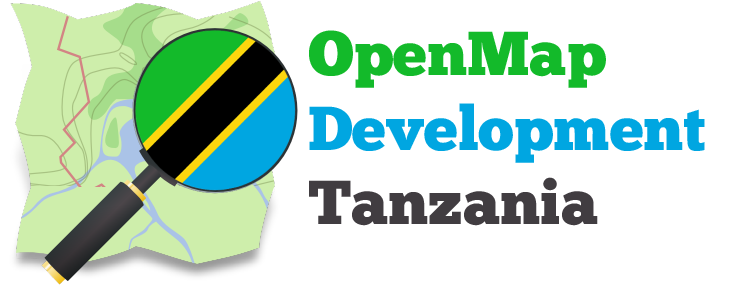
\includegraphics[width=4cm]{images/OpenMap_Development_TZ_Logo_Security_Card.png}}
  % \maketitle
}
\bigskip  \bigskip \bigskip
\begin{center}
  March 2019, Dar es Salaam, Tanzania  
  
 \bigskip \bigskip \bigskip \bigskip \bigskip \bigskip
\end{center}
 
\begin{flushleft}
	\footnotesize {\textbf{Authors:} Wombura Kimacha, Evarist Isdory, Johanes Peter, Hawa Adinani, Immaculate Mwanja and { } { } { } { } { } { } Innocent Maholi}
\end{flushleft} 
  

\newpage
\tableofcontents

\newpage
\section{Summary}
With the support from \href{http://www.hdif-tz.org/}{Human Development Innovation Fund}\footnote{\url{http://www.hdif-tz.org/}} (HDIF), OpenMap Development Tanzania has been working to develop an innovation map platform and adding in relevant features and plugins to make the platform user friendly and easy to interact with.  This report describes the second quarter of the Innovation Ecosystem Map of Tanzania Project. It provides an in-depth description of the activities done from April to July of 2019, what we have learned so far from the engagement with stakeholders and an evaluation of the sustainability models of the Innovation Ecosystem Map of Tanzania, and most importantly the development of the Web and how many innovators have been mapped.

\section{Milestones}
This section provides an overview of the project status with regards to conducted activities and their progress as well as describing the milestones:

\subsection{Web Development}
At the end of the first week of May, 2019 OMDTZ team started working on developing a new mapping platform that will replace the \href{http://innovate.co.tz}{previous innovation map platform}\footnote{\url{http://innovate.co.tz}}. Development of the new mapping platform was carried out for a period of almost two months. The following activities were done during the period:

\begin{itemize}
	\item Research for main layout,
	\item Concept generation, prototyping
	\item Development, and internal reviews to gain feedback
	\item External sharing and review with HDIF
\end{itemize}

On the fourth week of June, the new platform was completed awaiting reviews from the stakeholders during a mapathon. Now that the \href{http://new.innovate.co.tz}{new map}\footnote{\url{http://new.innovate.co.tz}} is accessible, below is the comparison of the looks between the two platforms:

\begin{figure}
	\caption{Old innovation ecosystem map}
	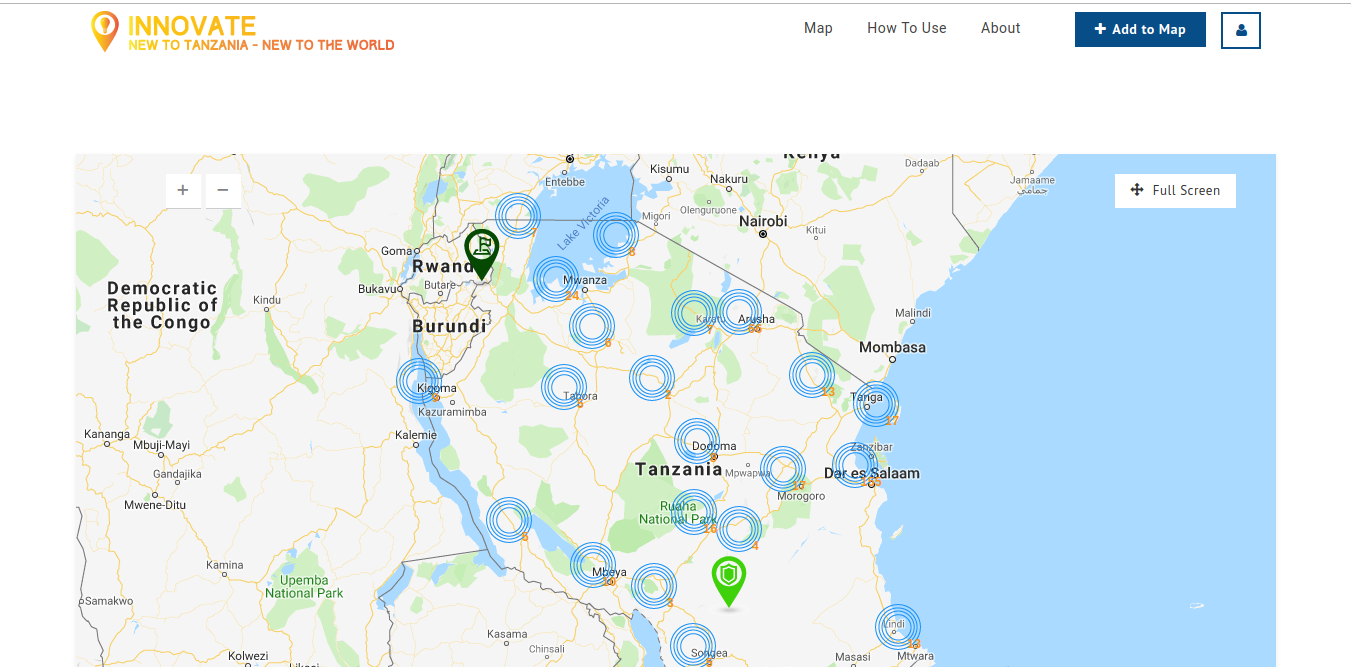
\includegraphics[width=0.9\textwidth]{old_inno_map.PNG}
	\
	\
	\
	\caption{New innovation ecosystem map}
	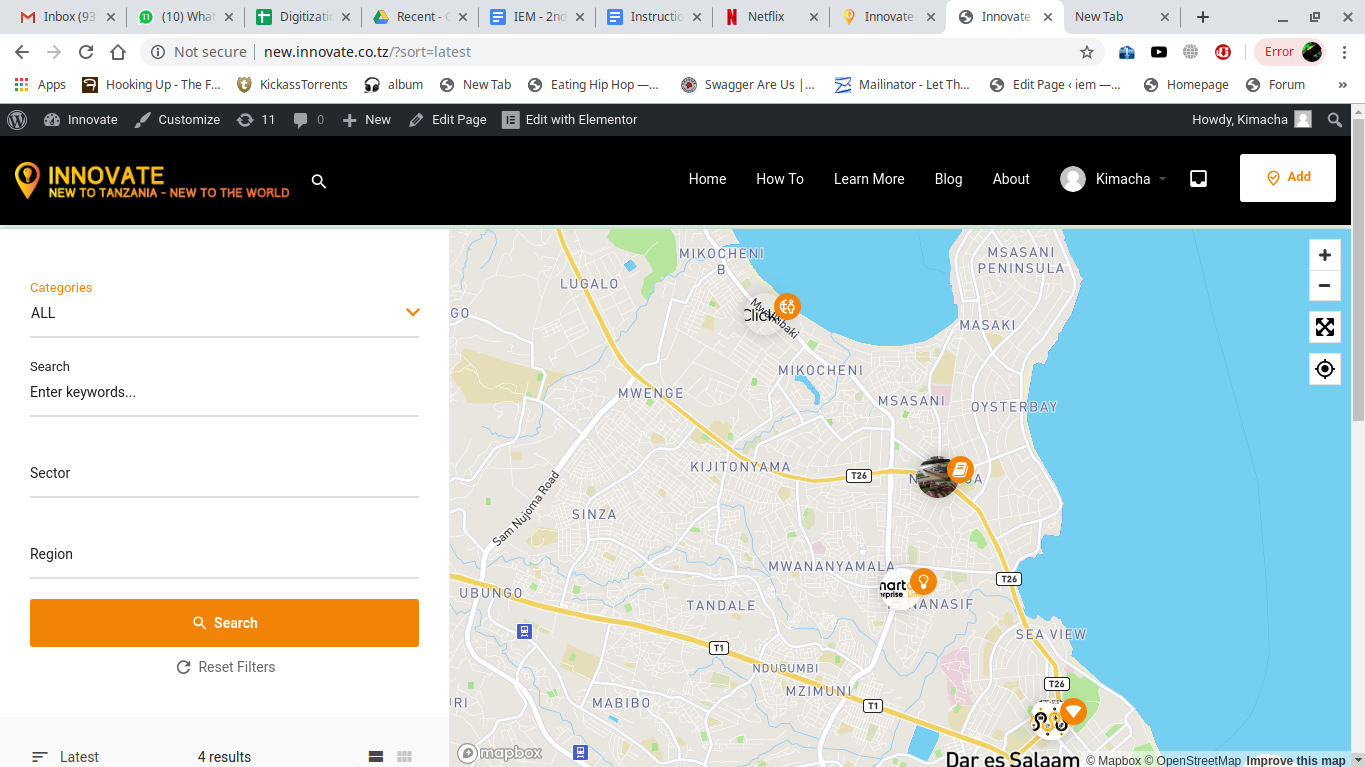
\includegraphics[width=0.9\textwidth]{new_inno_map.PNG}
\end{figure}

\newpage
\section{Training of Trainers}
OMDTZ in collaboration with HDIF, conducted training for the trainers which took place on July 15th, 2019 at OMDTZ’s offices. The objectives of the training were to train mappers how to conduct mapathons and introduce them to travel guidelines that should be followed while in the field and to provide supervision and technical support to conduct the Innovation Ecosystem Map of Tanzania project in districts or regions during data collection.

Following the training that were provided on January 2019, the trainers were already familiar with the categories and contents of the Innovation Ecosystem of Tanzania. The training was collaborative as it provided the room for interaction for every participant to make comments and suggestions on the stakeholders, categories, sub-categories, and targeted groups on the map. 

The training mainly focused on training the trainers who will be going out to the field all over Tanzania to hold mapathons and/or workshops with hub managers, innovators, teaching institutions, etc. in order to populate the map that is being developed.

The focus of the training was based on:

\begin{itemize}
	\item Introducing the trainers to the travel guidelines that should be followed when in the field in districts and regions
	\item How to conduct mapathons with involvement of innovation stakeholders in the districts and regions
	\begin{itemize}
		\item How to register stakeholders and adding the listings of their categories
		\item Facilitate stakeholders in conducting their own mapathons and workshops that will be attended by the innovation stakeholders that could not be reached by the trainers
	\end{itemize}
	\item Introducing the trainers to the web map developed for the innovation ecosystem of Tanzania
	\item Preparing and planning for the mapathon
\end{itemize}

The training of trainers was succeeded by a mapathon that was conducted the next day on July 16, 2019.

\begin{figure}[H] % uncomment "[H]" to force the  image to the middle of the page  
	\centering
	\caption{Training of trainers at OpenMap Development Tanzania offices}
	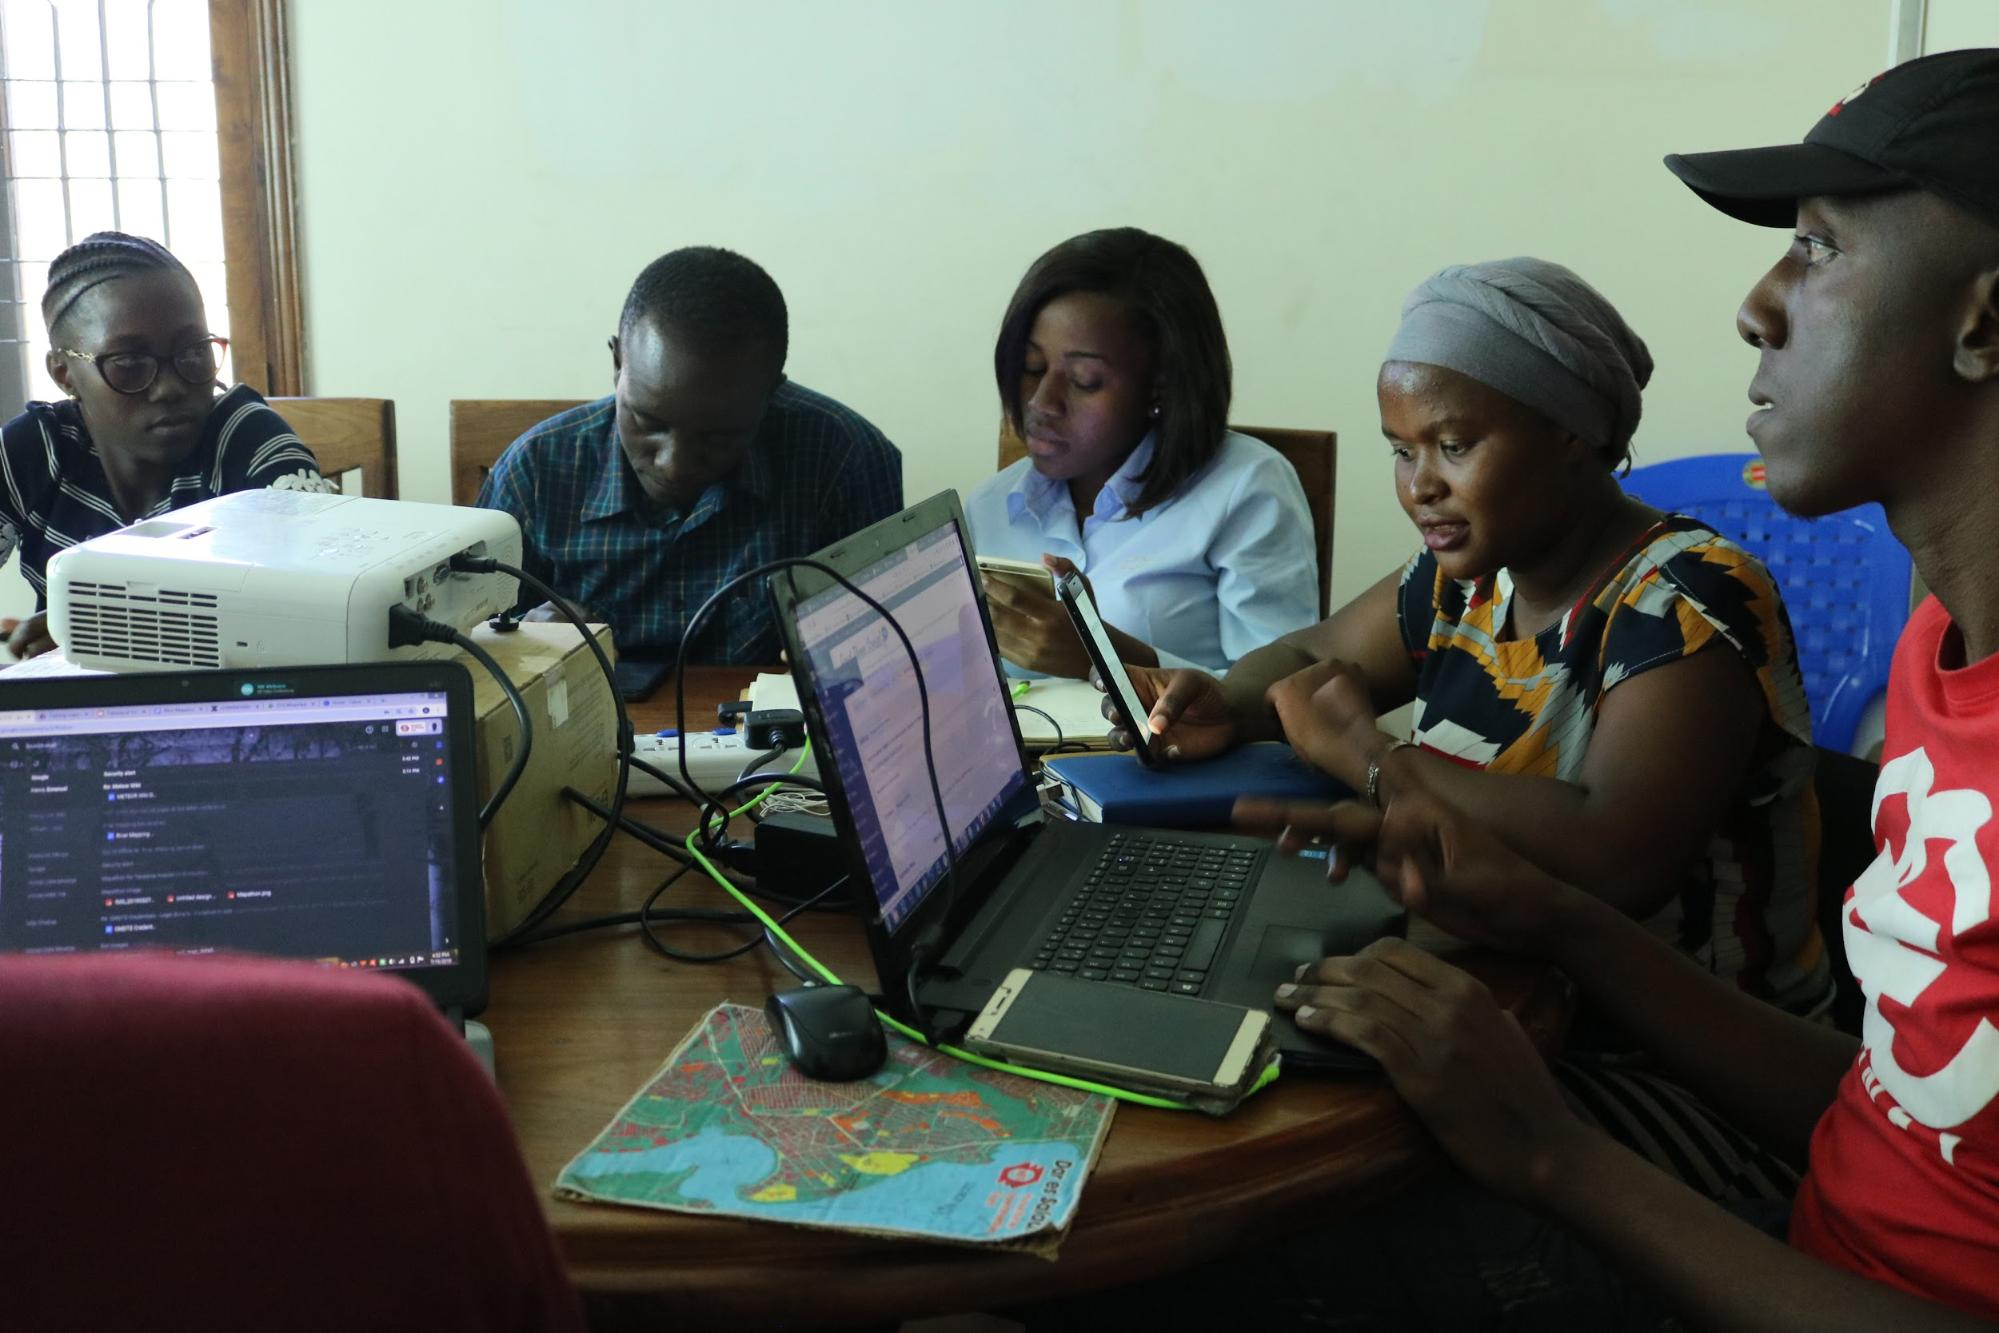
\includegraphics[width=0.9\textwidth]{training.JPG}
\end{figure}

\section{Mapathon}
This was a coordinated mapping event organized by OMDTZ with support from HDIF. The mapathon that was preceded by a training of trainers conducted the previous day, took place on July 16th, 2019 at Tanzania Data Lab and was attended by 14 stakeholders from various innovation backgrounds, trainers and staff from OMDTZ and facilitators from HDIF.

Participants of the mapathon were provided with Eventbrite tickets as notice prior to the mapathon in order to coordinate and prepare well. Before conducting a mapathon, OMDTZ contacted respective labs/hubs/university or any other physical innovation space in the Dar es Salaam that would participate in the mapathon.

The mapathon took approximately a maximum of 3 hours where the participants received full training on how to map themselves then use the time to actually map their organizations. What we learned is that most of the participants were familiar with the new map being developed by OMDTZ from the Hubs Manager’s workshop, exhibition, and presentations held during the Innovation Week of 25th - 30th of March, 2019. 

\begin{figure}%[H]
	\centering
	\caption{Mapathon conducted at Tanzania DataLab}
	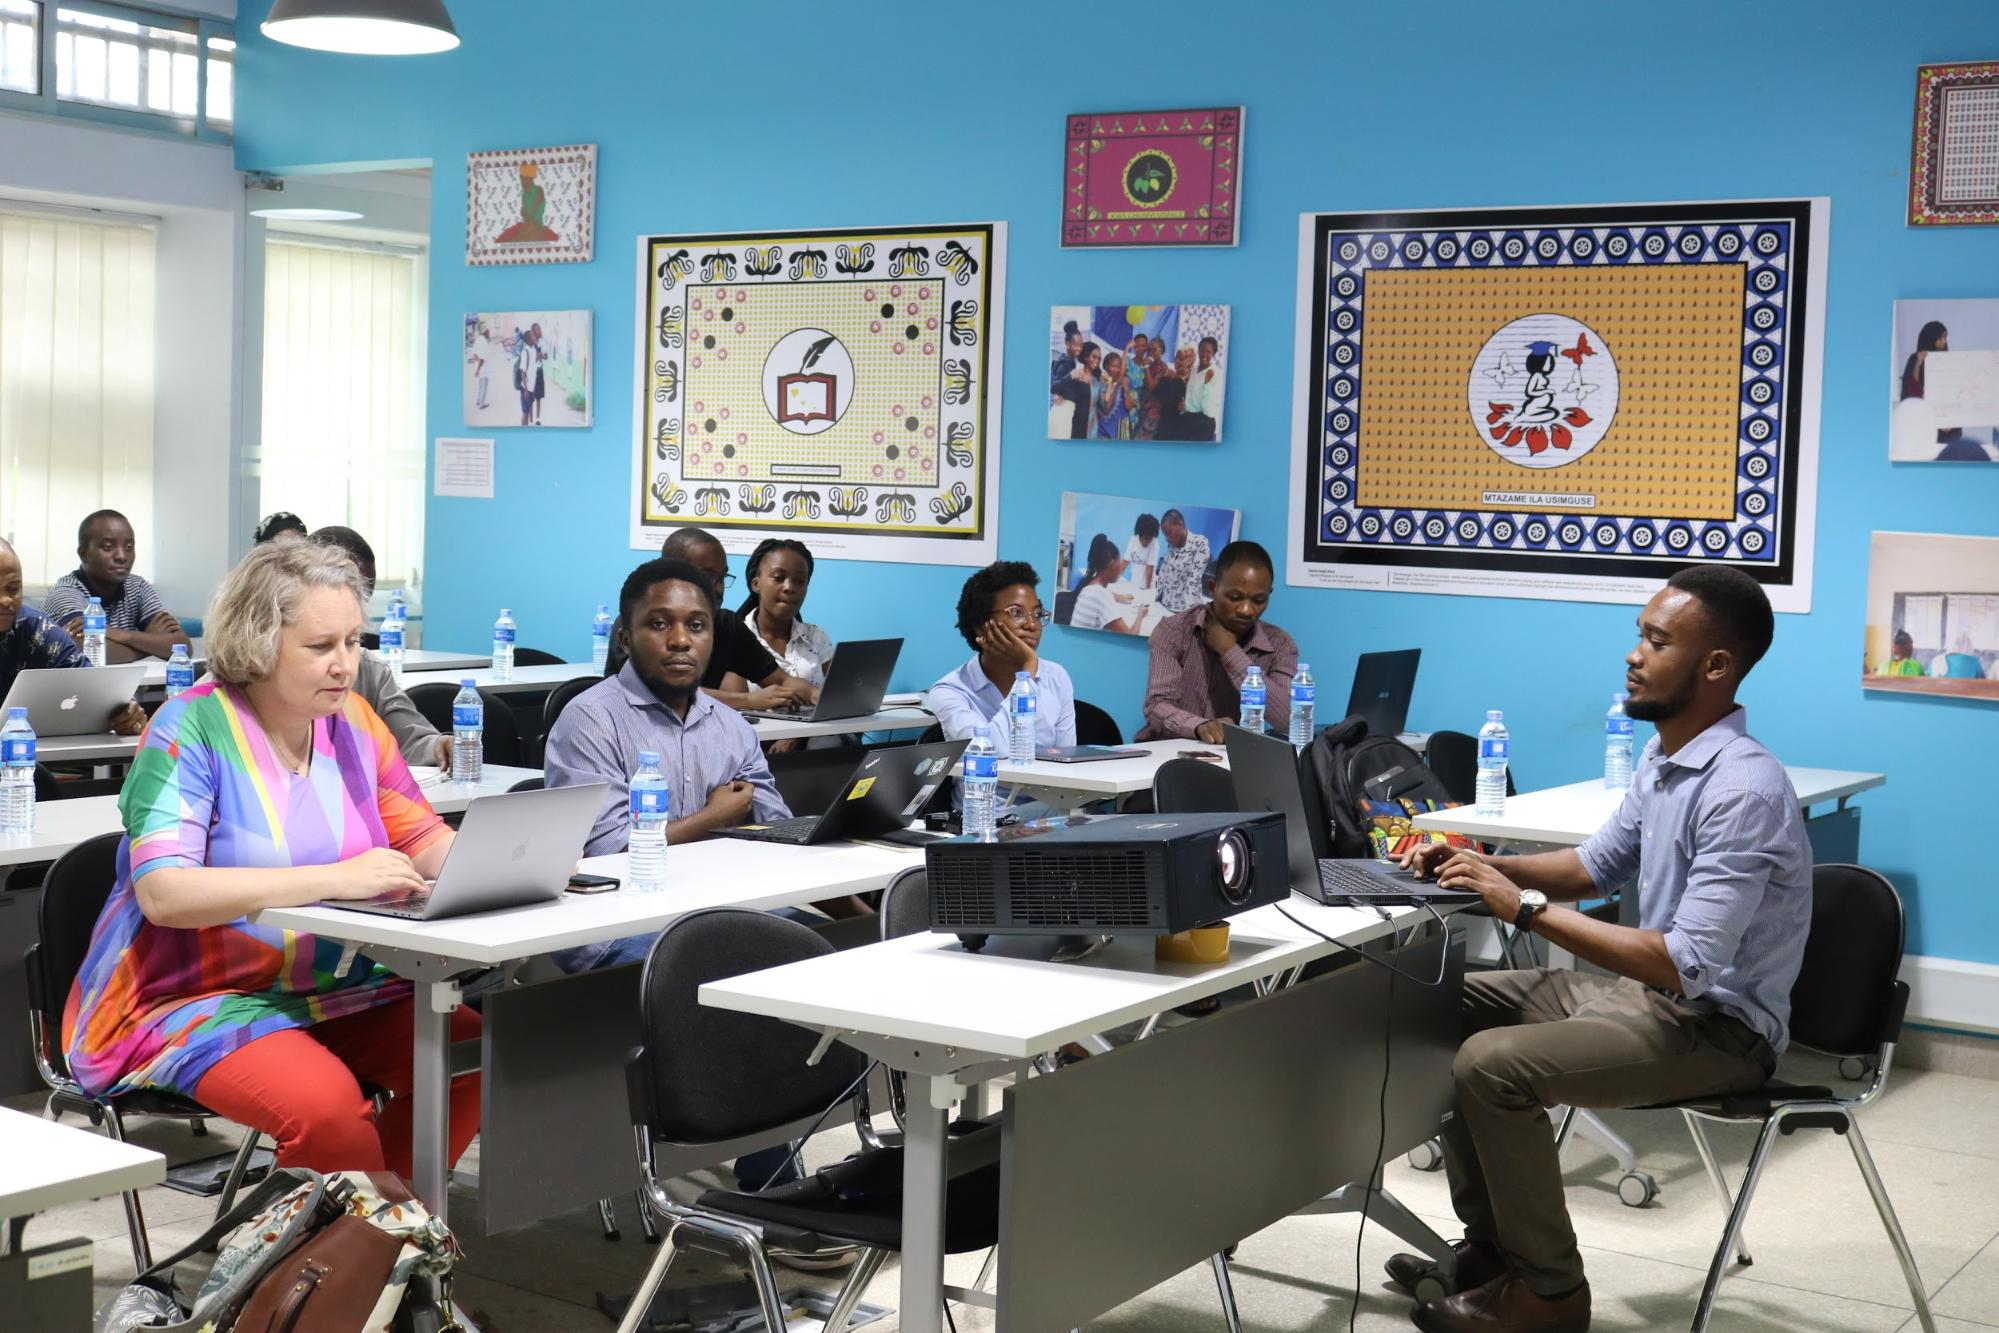
\includegraphics[width=0.85\textwidth]{mapathon.JPG}
\end{figure}

We got constructive feedback from the participants of the mapathon as all the attendees agreed that all the categories that have been provided on the map are exhaustive enough. By the end of the training, the participants were asked to give feedback reflecting on the whole event. We intend to collaborate with more innovation stakeholders in the mapathons and workshops that will be held in the future to improve and make the ecosystem map sustainable.

\section{Communications}
Communicating to the public about the map is the main thing that makes a map popular. We have prepared a communication strategy---just for the map. The strategy will guide all communications about the project and the type of content to be shared.

One blog draft has been developed but it has not been published as we are still waiting for reviews from HDIF's side. It will be published as soon as the article is reviewed.

Also, during the innovation week we had an opportunity to publicise the map to different stakeholders and featured on two media platforms---ITV news (we could not manage to get the link) and BBC News Swahili in Mitikasi Leo Show---where we introduced the map and explain why HDIF is interested on this platform and how it will be useful to the ecosystem of Tanzania's innovation.

\subsection{Social Media}
We managed to create Facebook and \href{https://twitter.com/innovate_tz}{Twitter}\footnote{\url{https://twitter.com/innovate_tz}} accounts and we have started posting about the Map. We have 63 followers on Twitter and some work and extra effort is needed in order to boost our followers and engagement on social media. 

We decided---with advice from HDIF---to create only two social media account for some reasons:

\begin{enumerate}
	\item Handling multiple accounts is challenging especially when the accounts are not popular yet.
	\item Being able to create good and reliable contents becomes easy with lesser accounts
\end{enumerate}

\section{Learning and Challenges}
\subsection{Web Platform}
\subsection{Mapathon}

\section{Financial Reporting}
The financial report for this project can be accessed:


\end{document}
